%-------------------------------------------------------------------------------------------------------
%-------------------------------------------------------------------------------------------------------
% Sec & Label

\section{Simulation Analysis}
\label{sec:simulation}


%-------------------------------------------------------------------------------------------------------
%-------------------------------------------------------------------------------------------------------
% Intro

In this section, Circuit T4 is reproduced with the help of Ngspice.

Ngspice is a simulator for eletronic circuits that can output a variety of results.
This emulator computes the voltages in every node, as well as the potential difference
between two given nodes. Apart from that, the group made use of the command
{\em .options savecurrents} which also enables the use of the currents that pass
through all branches. Moreover, function to help determine the maximum and interception
of the plots were also used.

Firstly, the outcome of the simulation is shown, as well as a brief explanation
on how it was achived. Afterwards, a comparison is done between those values and
the ones attained in Section \ref{sec:analysis}.



%-----------------------------------------------------------------------
%-----------------------------------------------------------------------
% 			     Results - subsec
% ----------------------------------------------------------------------
% ----------------------------------------------------------------------

\subsection{Simulated results}
\label{subsec:sim_res}

In this laboratory assignament, the Ngspice script made use of the sames values considered for the Octave script.

Table \ref{tab:imp_sim} dislpays the total impedances of the circuit (Input and Output). These are attained by dividing the potencial difference of the sinusoidal voltage source by the current that passes through it at a reasonble instant.

For the Outup impedance a small change in the circuit was done. The original sinusoidal voltage source is connected to the "out" node of the OP-AMP and Ground,a nd in its inicial position is now a short-circuit. Optimally this value should be as close to zero as possible, such is not verified because of the need to improve the Merit. 

\begin{table}[ht]
	\centering
	\begin{tabular}{|l|r|}
		\hline    
		{\bf Name} & {\bf Value[Ohm]} \\ \hline
    		Zin & 923.912\\ \hline

    		Zout & 522.442 + -316.233 j\\ \hline
Abs(Zout) & 610.695\\ \hline

	\end{tabular}
	
	\caption{Total impedance values from Ngspice.}
    
\label{tab:imp_sim}
\end{table}

Figure \ref{fig:Vout} displays $vdb_{out}$ (in decibels) from 10Hz to 100MHz, as well as a constant ($max-3(dB)$) - this helps to better visualize the passband. The $vdb_{out}$ curve is characteristic of a band pass filter (cutting high and low frequencies).

\begin{figure}[ht]
	\centering
	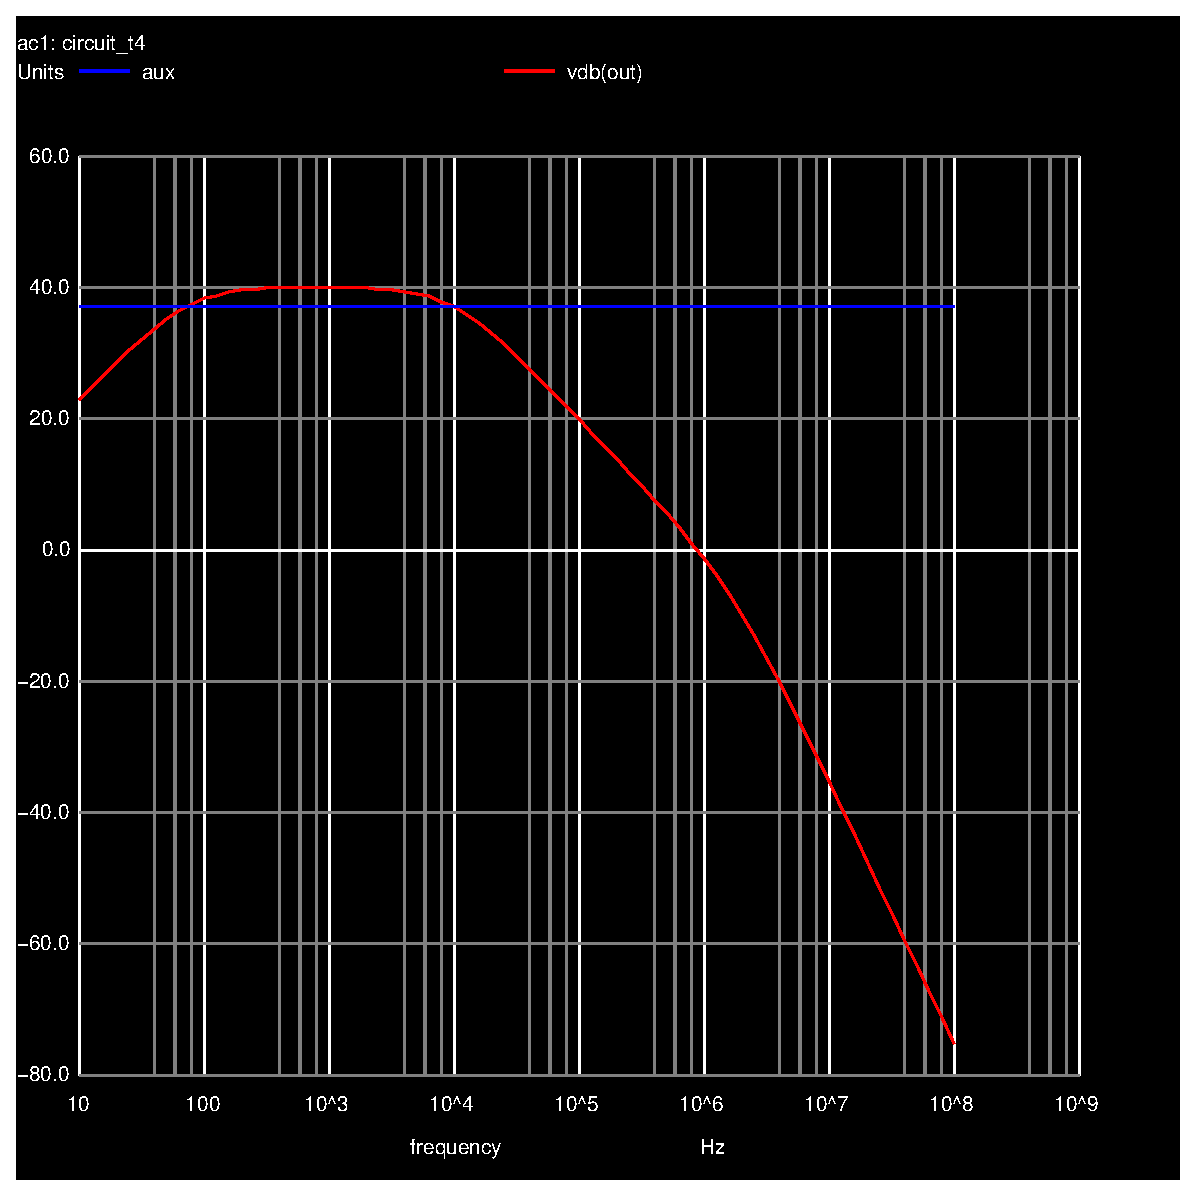
\includegraphics[width=0.6\linewidth]{acvout.eps}
	\caption{$vdb_{out}$}
\label{fig:Vout}
\end{figure}

This graph is of particular importance because it allows us to obtain the GainDeviation. This is simply given by the absolute value of ($Maximum - 100$), 40db or 100 (linearly) being the Gain at central frequency. Therefore, the closest the maximum of said graph is to 40dB, the lower its deviation is and the higher the Merit will be. This variable has no units.

Moreover, with the plot in Figure \ref{fig:Vout}, we were able to measure the Central frequency. This variable is given by: 

\[
CentralFreq = \sqrt(LowerFreq\times UpperFreq) 
\]

The {\emph LowerFreq} and {\emph UpperFreq} are the frequencies of the intersection points of the $vdb_{out}$ curve and its max minus $3$. Its deviation is {\emph CentralFreq}$-1000$. This variable is given in Hertz (Hz).

%\begin{figure}[ht]
%	\centering
%	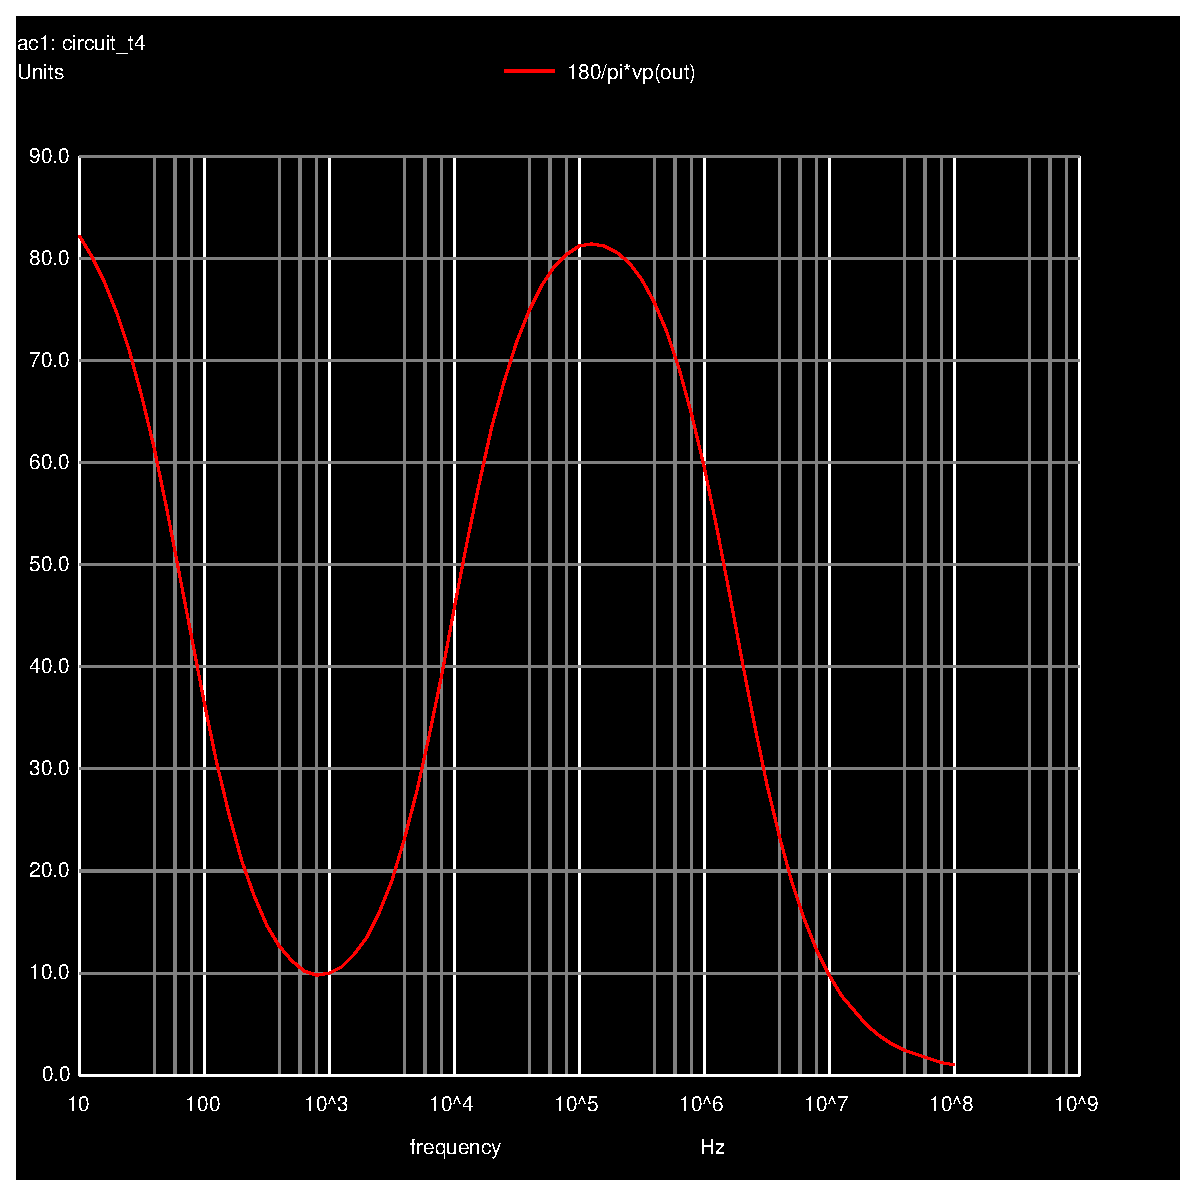
\includegraphics[width=0.6\linewidth]{phasevout.eps}
%	\caption{$vdb_{out}$}
%\label{fig:Vout}
%\end{figure}

Lastly, the group also used Ngspice to compute the Merit. Table \ref{tab:merit} shows all the 
values necessary to compute the Merit, as well as the Merit itself. Note that the total cost is the sum 
of the costs of resistors, capacitors and transistors of the total circuit (including de OP-AMP).

\begin{table}[ht]
	\centering
	\begin{tabular}{|l|r|}
		\hline    
		{\bf Name} & {\bf Value} \\ \hline
    		cost & 1.343451e+04\\ \hline
gain & 1.003168e+02\\ \hline
gaindev & 3.167835e-01\\ \hline
centralfreq & 8.476811e+02\\ \hline
centralfreqdev & 1.523189e+02\\ \hline
 ---------- & -------------------- \\ \hline
merit & 4.876656e-07\\ \hline

	\end{tabular}
	
	\caption{Merit and other variables.}
    
\label{tab:merit}
\end{table}

